
\begin{table}[!htbp]
\centering
\caption{Details of the seven investigated plan configurations.}
\label{tab:investigated_models}
\small
\resizebox{\textwidth}{!}{%
\begin{tabular}{@{}llccc p{4.0cm}@{}}
\toprule
Model & Plan type & Storeys & Plan area (m$^2$) & GII (\%) & Special feature \\
\midrule
Regular & Rectangular & 3 + stair cover & 72 & 0.00 & Reference rectangular plan \\
L & L-shaped & 3 + stair cover & 60 & 16.67 & Single re-entrant corner \\
L1 & L-shaped & 3 + stair cover & 48 & 33.33 & Deeper single re-entrant corner \\
L2 & Stepped L-type & 3 + stair cover & 72 & 33.33 & Two-step re-entrant topology \\
T & T-shaped & 3 + stair cover & 48 & 33.33 & Two re-entrant corners \\
U & U-shaped & 3 + stair cover & 60 & 16.67 & Central notch and two re-entrant corners \\
Non-Parallel & Skewed & 3 + stair cover & 84 & 22.22 & Non-parallel framing; $\theta=36.87^{\circ}$ \\
\bottomrule
\end{tabular}
}
\end{table}

% The source floor-plan PDFs are full-page Letter drawings.  CP112 previously used a
% large hard-coded bottom trim, which clipped the lower half of the plans.  These calls
% use tightly cropped vector derivatives so the complete drawings remain visible.
\begin{figure}[H]
\centering
\begin{subfigure}[t]{0.49\textwidth}\centering
\includegraphics[width=\linewidth,keepaspectratio]{figures/ch3/floor_plans/regular_floor_plan.pdf}
\subcaption{Regular}
\end{subfigure}\hfill
\begin{subfigure}[t]{0.49\textwidth}\centering
\includegraphics[width=\linewidth,keepaspectratio]{figures/ch3/floor_plans/l_floor_plan.pdf}
\subcaption{L-shaped}
\end{subfigure}
\caption{Regular and L-shaped floor plans.}
\label{fig:floorplans_regular_l}
\end{figure}

Figure~\ref{fig:floorplans_regular_l} compares the regular reference plan with the first re-entrant L-shaped configuration. The pair provides a direct geometric basis for examining how the introduction of a re-entrant corner changes the plan while the broader modelling framework remains common.


\begin{figure}[H]
\centering
\begin{subfigure}[t]{0.49\textwidth}\centering
\includegraphics[width=\linewidth,keepaspectratio]{figures/ch3/floor_plans/l1_floor_plan.pdf}
\subcaption{L1-shaped}
\end{subfigure}\hfill
\begin{subfigure}[t]{0.49\textwidth}\centering
\includegraphics[width=\linewidth,keepaspectratio]{figures/ch3/floor_plans/l2_floor_plan.pdf}
\subcaption{L2-shaped}
\end{subfigure}
\caption{L1- and L2-shaped floor plans.}
\label{fig:floorplans_l1_l2}
\end{figure}

Figure~\ref{fig:floorplans_l1_l2} shows that the L1 and L2 configurations represent different re-entrant geometries rather than simple scaled copies. Their separate treatment is necessary because equal or similar area-deficit measures do not preserve the location and topology of the missing plan area.


\begin{figure}[H]
\centering
\begin{subfigure}[t]{0.49\textwidth}\centering
\includegraphics[width=\linewidth,keepaspectratio]{figures/ch3/floor_plans/t_floor_plan.pdf}
\subcaption{T-shaped}
\end{subfigure}\hfill
\begin{subfigure}[t]{0.49\textwidth}\centering
\includegraphics[width=\linewidth,keepaspectratio]{figures/ch3/floor_plans/u_floor_plan.pdf}
\subcaption{U-shaped}
\end{subfigure}
\caption{T- and U-shaped floor plans.}
\label{fig:floorplans_t_u}
\end{figure}

Figure~\ref{fig:floorplans_t_u} presents two configurations with multiple re-entrant corners. The T- and U-shaped plans distribute the removed area differently, which can alter stiffness distribution, eccentricity and deformation demand even when a single area-based index is similar.


\begin{figure}[H]
\centering
\includegraphics[width=0.86\textwidth,height=0.42\textheight,keepaspectratio]{figures/ch3/floor_plans/non_parallel_floor_plan.pdf}
\caption{Non-Parallel floor plan.}
\label{fig:floorplan_nonparallel}
\end{figure}

Figure~\ref{fig:floorplan_nonparallel} shows the skewed framing arrangement of the Non-Parallel configuration. Its geometric mechanism differs from the re-entrant-corner cases, so the non-parallel angle is retained separately from the area-deficit GII.

\FloatBarrier

\subsection{Geometric Irregularity Index Definition}
For the plan comparison, GII is the percentage plan-area deficit relative to the corresponding bounding rectangle. Figure~\ref{fig:gii_definition} shows the definition schematically for a re-entrant plan. The missing/re-entrant area is a geometric descriptor only; the location and topology of the missing area are retained separately through the plan type, re-entrant projections and corner count.

\begin{figure}[!htbp]
\centering
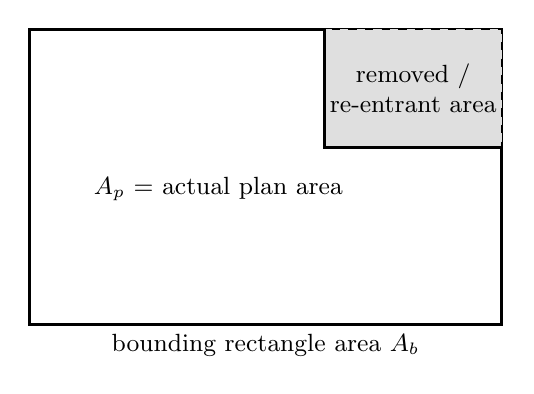
\begin{tikzpicture}[scale=0.75,font=\small]
\draw[very thick] (0,0) rectangle (8,5);
\fill[gray!25] (5,3) rectangle (8,5);
\draw[very thick] (0,0)--(8,0)--(8,3)--(5,3)--(5,5)--(0,5)--cycle;
\draw[dashed] (0,0) rectangle (8,5);
\node at (3.2,2.3) {$A_p$ = actual plan area};
\node[align=center] at (6.5,4.0) {removed /\\re-entrant area};
\node[below] at (4,0) {bounding rectangle area $A_b$};
\end{tikzpicture}
\caption{Geometric Irregularity Index definition.}
\label{fig:gii_definition}
\end{figure}

Figure~\ref{fig:gii_definition} defines GII as the percentage difference between the bounding-rectangle area and the actual plan area. The index therefore measures plan-area deficit only; it does not identify the location, direction or topology of the irregular portion.


\begin{table}[!htbp]
\centering
\caption{Geometric descriptors used with GII.}
\label{tab:gii_geometry}
\scriptsize
\resizebox{\textwidth}{!}{%
\begin{tabular}{@{}lcccccccc@{}}
\toprule
Model & $A_p$ & $A_b$ & GII & corners & max $R_x$ & max $R_y$ & aspect & $\theta$ \\
 & (m$^2$) & (m$^2$) & (\%) & & (\%) & (\%) & ratio & (deg) \\
\midrule
Regular & 72 & 72 & 0.00 & 0 & 0.00 & 0.00 & 2.00 & -- \\
L & 60 & 72 & 16.67 & 1 & 33.33 & 50.00 & 2.00 & -- \\
L1 & 48 & 72 & 33.33 & 1 & 66.67 & 50.00 & 2.00 & -- \\
L2 & 72 & 108 & 33.33 & 2 & 33.33 & 33.33 & 1.33 & -- \\
T & 48 & 72 & 33.33 & 2 & 33.33 & 50.00 & 2.00 & -- \\
U & 60 & 72 & 16.67 & 2 & 33.33 & 50.00 & 2.00 & -- \\
Non-Parallel & 84 & 108 & 22.22 & 0 & 0.00 & 0.00 & 1.33 & 36.87 \\
\bottomrule
\end{tabular}
}
\par\smallskip
\begin{minipage}{0.97\textwidth}\footnotesize
$R_x$ and $R_y$ are geometric re-entrant projection descriptors used in the geometric calculations; they are kept distinct from GII. The Non-Parallel angle is an additional study descriptor and is not folded into GII.
\end{minipage}
\end{table}
\FloatBarrier
